\documentclass[letterpaper, 12pt]{article}
%\documentclass{tufte-book}
\usepackage{color}
\usepackage{graphicx}
% Color boxes - nice
\usepackage[most]{tcolorbox}
% I like smaller margins
\usepackage[margin=1.0in]{geometry}
% Corporate speak, make a paragraph of bullshit
\usepackage{lipsum}


% Log entries
\newenvironment{loggentry}[2]% date, heading
{\noindent\textbf{#2}\hspace{\parindent}\textbf{#1}\\}

\begin{document}

\title{Use of Temperature Compensation for Single Dish Total Power Observations}
\author{Dave Cohen}
\date{August 2, 2021}
\maketitle

\pagenumbering{roman}
\tableofcontents
\newpage
\pagenumbering{arabic}

\section{Introduction}
Many of the components used in a radio telescope are very sensitive to temperature. This is especially true of the LNA (Low Noise Amplifier), where adding temperature compensation can result in the degradation of noise figure of the LNA {\color{red}(any evidence to support this?)}. This is one of the major challenges to total power measurements, as the change in output of the receiver due to temperature is typically much greater than the change due to an actual source.

Serveral attempts have been made by the author to stabilize the temperature of the front-end components of the telescope, with varying degrees of success. These usually involve an insulated chamber that houses the components, and a temperature control system involving a heating or cooling device that usually consists of a Peltier junction. If cooling/heating is done in conjunction with a temperature sensor in a closed-loop control system, temperature regualation within +/- 0.1 degree Celcius has been achieved.

The problem with temperature control is mainly with the complexity of the system, and the number of components. The following devices as a minimum would be required:

\begin{itemize}
	\item[-] Temperature sensor for feedback
	\item[-] Processor to determine error and provide drive to amplifier
	\item[-] Amplifier to drive the Peltier junction
	\item[-] A fair amount of power supply to drive the Peltier amplifier
	\item[-] The Peltier junction
	\item[-] Insulated enclosure to reduce demand on the control system
\end{itemize}

In addition to the complexity of the temperature control, problems can arise from improper control of temperature. Crossing the dew point when using cooling can cause condensation, which can be harmful to electronics, as well as excessive heat. An LNA generates heat on its own, which causes further complications.

In order to avoid a lot of the problems previously discussed, an attempt will be made to remove the effects of temperature without any temperature control other than an insulated encloure to reduce temperature fluctuations. This should be possible with an accurate temperature sensor and a mathematical model of the temperature response of the entire receiver system.

\section{Determining Temperature Response of the System}
Before the temperature response of the system can be determined, it is necessary to have accurate temperature measurements of the system. It will also be necessary to have the ability to subject the system to the temperature ranges that it will undergo during normal operation. To that end, some equipment will need to be acquired.

\subsection{Temperature Measurement Equipment}
There are some excellent low-cost options for temperature measurement available. 

\begin{itemize}
	\item[-] Platinum PT100 RTD three-wire temperature sensor. 
	\\Platinum sensors are supposed to have higher accuracy and stability 			than thermocouples. They have a 100-ohm resistance at 0 degrees C, and 			vary reisistance at the rate of 0.385 ohms per degree C. The third wire 	is used as a voltage sense wire to compensate for lead length. The 				Adafruit 3290 will be used for this purpose.
	\item[-] Temperature sensor amplifier.
	\\Adafruit 3328, a MAX31865 RTD amplifier will be used to diigtize the 			signal.  It uses SPI (Serial Peripheral Interface) to transmit 					temperature data to a controller.
	\item[-] Arduino Nano.
	\\A tiny, low-cost controller that will communicate with the MAX31865 			via SPI.  The Nano will communicate with a computer over USB, which 			will also provide power to the Nano.  A library using a high-accuracy 			lookup table is available at \\
	https://github.com/drhaney/pt100rtd
\end{itemize}

\subsection{Thermal Testing}
An insulated enclosure must be provided to both minimize temperature fluctuations, and to provide an environment where temperature can be changed in a controlled manner. The enclosure must be of sufficient size to house all of the receiver components, from front end to computer.  Weatherproof coolers are being evaluated for this purpose.

Thermal testing will be done as follows:

\begin{itemize}
	\item[-] Ice (or dry ice?) in a tray will be bring the temperature down 		the low extreme, where the test will be started. The ice will be allowed 	to melt (or sunlimate).
	\item[-] A source of heat will be placed in the cooler.  An incandescent 	bulb and fixture controlled by a dimmer are being considered for this 			purpose.
\end{itemize}
 

\section{Journal}


\begin{loggentry}{2021-08-11}{Parts Arrived}

Received parts and wired MAX31865 RTD amplifier and RTD. Had trouble with tiny solder jumpers on eval. board. Also had a lot crashed in Arduino IDE on Raspberry Pi, especially when connected to serial monitor.  Ended up moving to NUCRA mini computer to get hardware working. Got Adafruit software working, but I moved on to the more precise software offered on (github ref), which uses a lookup table which supposedly provides the most accurate temperature readings.  I got that software working as well.  I am now just starting to modify the Arduino code to listen to the serial port. A python test application has been created.  My next problem is to properly parse the usb devices to locate the serial port for the Nano. I think that I am doing this wrong for the USB relay in tp\_soapee.py, but it happens to be working because it occurs as the first device, which I have hardcoded.  That needs to get fixed when I bring in the new code for temperature measurement.
\\
\end{loggentry}


\begin{loggentry}{2021-08-13}{Plotting Temperature}

Got software temperature logging working on Arduino and plotting working on Python.  Graph looks good and I have a few extra features, like subplots with varying height ratios.

\begin{figure}[h!]
	\centering
	%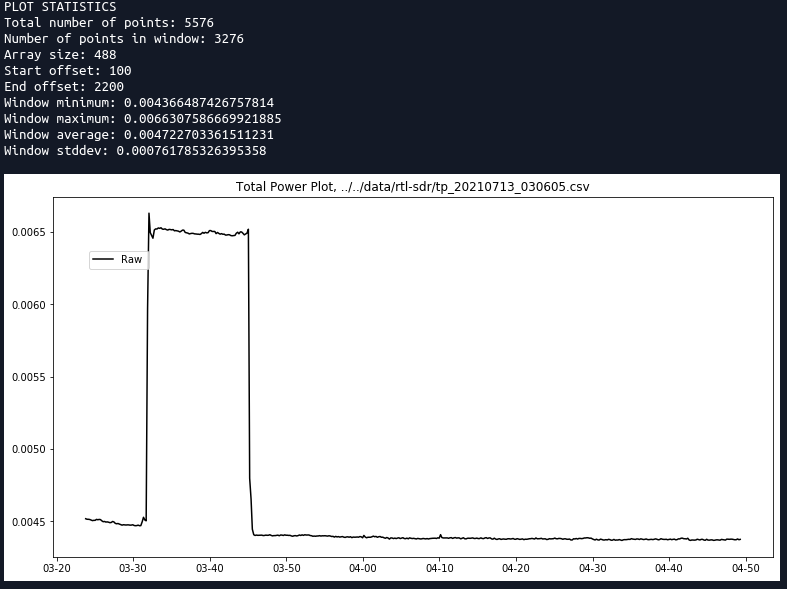
\includegraphics[width=1\textwidth]{tp_20210713_030605.png}
	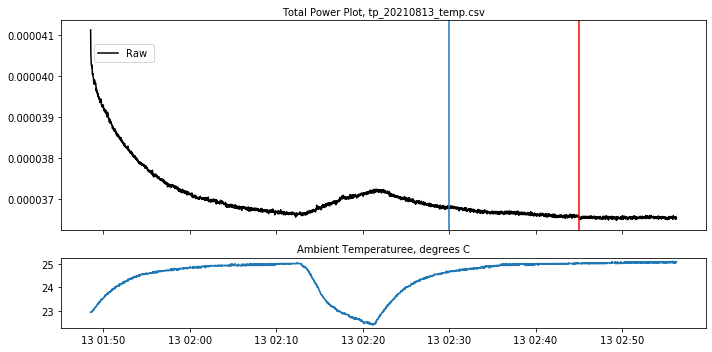
\includegraphics[width=1\textwidth]{temp_plot.png}
	\label{tplot}
	\caption{Total power with temperature plot.}
\end{figure}

There is a direct and obvious correlation between temperature and output visible when plotting this way. I hope that the resolution of the RTD and amplifier is sufficient to provide smooth temperature compensation.

The next step is to develop a temperature compensation method.  The current idea is to write a separate script that guides the user through the process. It could go something like this:

\begin{itemize}
	\item[-] Electronics warmup 
	\\Pause for a minimum warmup time, running the hardware but ignoring 			data.  This should be for a minimum of 90 minutes. 
	\item[-] Cooldown
	\\Place a cold substance (dry ice preferred) in the container with the 			hardware, taking necessary precautions. 
	\item[-] Warmup
	\\An incandescent bulb or other heat souce is placed in the container.
\end{itemize}

Are these separate recordings or one continuous one?  How will data be marked?  It's probably a bad idea to use rapid temperature changes, as thermal lag may be a factor. So the best method might be to house the electronics in a well insulated cooler with dry ice, and place it outside (sun or shade?). Allow the temperature to slowly climb to around 40 $^{\circ}$C, and stop recording.

Post-processing would entail creating temperature and output arrays that are on even temperature intervals, distributed through the entire temperature range. A curve fit would be done through the data, and each quantity plotted. This should result in an equation that could be fed back into the total power plotting program (how?). An additional command-line option would be added to allow for temperature compensation.  
\\
\end{loggentry}

\begin{loggentry}{2021-08-15}{Temperature Calibration, Take One}

Rough temperature calibration developed, using the following steps:

\begin{itemize}
	\item[-] CSV file loaded into pandas dataframe.
	\item[-] Time, total power, and temperature columns extracted and 				converted to Numpy arrays time\_array, tp\_array, and 							temperature\_array.
	\item[-] Based on the starting and ending offsets, existing arrays 				sliced to create new arrays time\_array\_window, tp\_array\_window, and 	temperature-array-window. These arrays will be used to calculate the 			temperature compensation curve.
	\item[-] Temperature window array is sorted by ascending temperature. 			Total power window array is sorted by temperature to maintain the one-			to-one correspondence between the temperature and total power.
	\item[-] New temperature array temperature\_array\_uniq created from 			unique values of temperature from the sorted array. Correspondig total 			power array tp\_array\_uniq created.
	\item[-] A curve-fit polynomial of order 3 is created from the unique 			temperature and total power arrays. This is assigned to the variable f.
	\item[-] The temperature compensated total power array is created by 			iterting through the original total power array tp\_array, and 					subtracting the returned value of f for the frequency corresponding to 			the total power value.
\end{itemize}

A three-hour run was made with the air conditioning cycling several times. A Noise calibrator signal was injected between 1700 and 1730 UTC. The results can be seen in figures~\ref{tcomp:1},~\ref{tcomp:2}, and~\ref{tcomp:3}:

\begin{figure}[h!]
	\centering
	%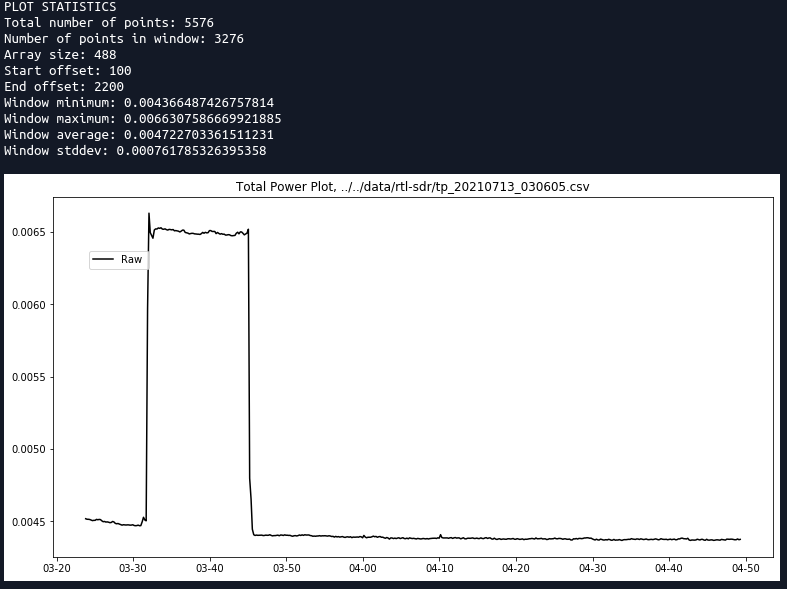
\includegraphics[width=1\textwidth]{tp_20210713_030605.png}
	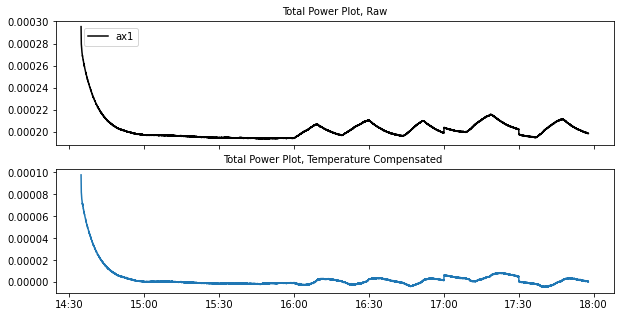
\includegraphics[width=1\textwidth]{tcomp20200815-1.png}
	\label{tcomp:1}
	\caption{Total power, raw and temperature compensated.}
\end{figure}

\begin{figure}[h!]
	\centering
	%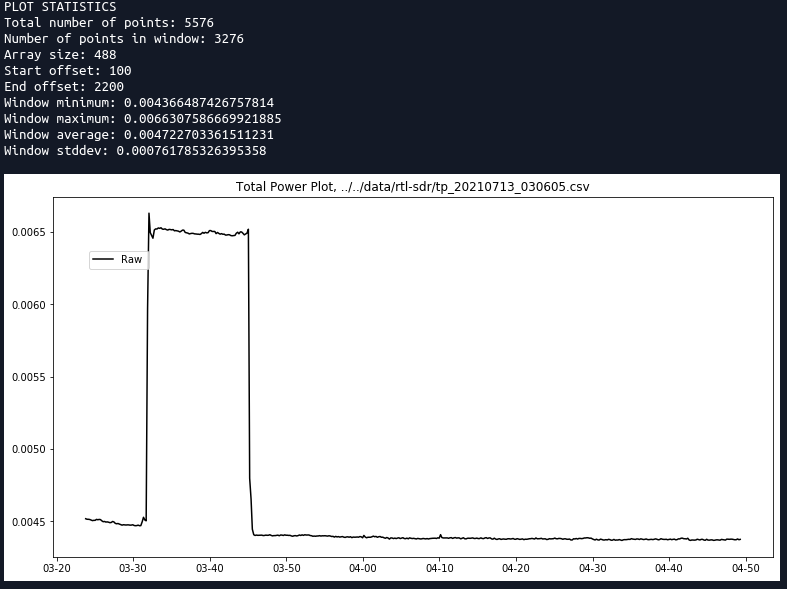
\includegraphics[width=1\textwidth]{tp_20210713_030605.png}
	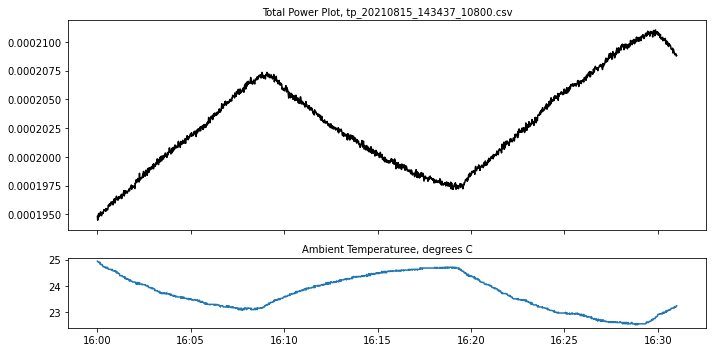
\includegraphics[width=1\textwidth]{tcomp20200815-2.png}
	\label{tcomp:2}
	\caption{The segment of the graph defined as the evaluation window, 			which is used to determine the temperauture/power correlation.}
\end{figure}

\begin{figure}[h!]
	\centering
	%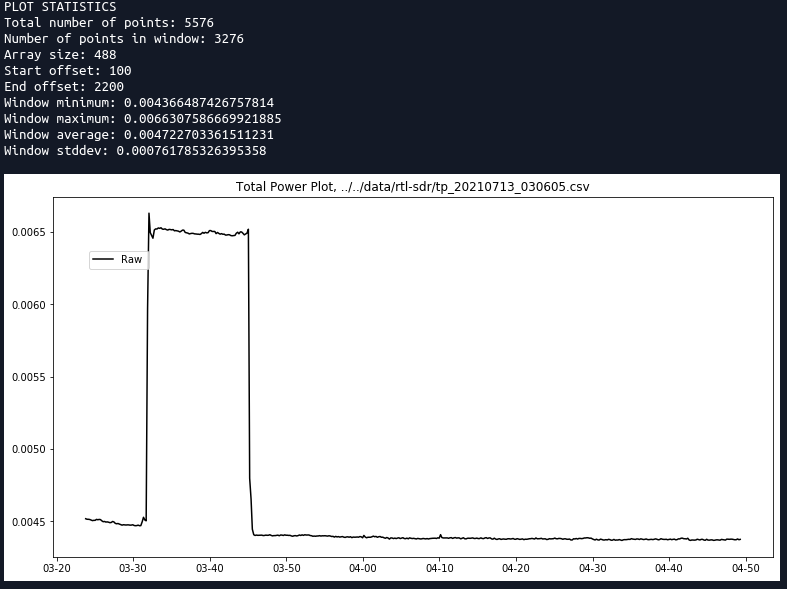
\includegraphics[width=1\textwidth]{tp_20210713_030605.png}
	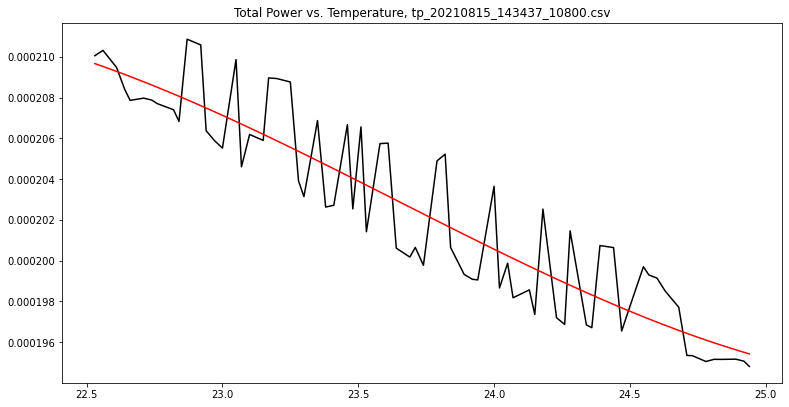
\includegraphics[width=1\textwidth]{tcomp20200815-3.png}
	\label{tcomp:3}
	\caption{The relationship between temperature and power. The curve fit 			function is shown in red.}
\end{figure}

It can be seen that there is a reduction of the change in signal by the contribution of temperature.  The contribution in signal by the noise source seems to be unaffected. Unfortunately, this is not effective enough to be called a success. A radio source could easily be masked by the curves in Figure~\ref{tcomp:1}; stronger sources being distorted by their presence.

The failure of this process to completely remove the termperature contribution is thought to be caused by the fact that for multiple measurements of the same temperature, the total power corresponding to each measurement can differ. Table \ref{table:1} shows the relationship between multiple measurements at a constant temperature, and the corresponding total power readings. These values are from the first six elements of temperature\_array\_sorted and tp\_array\_sorted. Some quick math on these values indicate a 0.22\% change from minimum to maximum values in this range.  That's a pretty small change, but that might not be typical for all temperature values. Looking at Figure ~\ref{tcomp:3} on the left side of the graph, the power values are very close to the polynomial curve. That is not the case for the values in the middle of the curve.

\begin{table}[h!]
\centering
\begin{tabular}{||l|l||} 
 \hline
 Temperature & Total Power \\ [0.5ex] 
 \hline\hline
 22.53 & 0.000210056 \\ 
 \hline
 22.53 & 0.000209956 \\
 \hline
 22.53 & 0.00021007  \\
 \hline
 22.53 & 0.000210417 \\
 \hline
 22.53 & 0.000210384 \\ 
 \hline
 22.53 & 0.00021006 \\
 \hline
\end{tabular}
\caption{Temperature and corresponding total measurements for multiple occurences of a single temperature.}
\label{table:1}
\end{table}

So what to do? A general statement could be made that the curve fit function isn't "strong" enough - it consistently doesn't remove enough of the temperature contribution, which might indicate that polynomial has the right slope, but the wrong offset in the y direction. But looking at Figure ~\ref{tcomp:3}, the power values vary on both sides of the polynomial curve. Applying smoothing to the total power array does not noticable improve the outcome. Applying smoothing to the temperature array causes more distortion in the total power output. I am considering averaging all the total power readings for a given temperature, and constructing the unique arrays from that. At least the total power values won't be at a minimum or maximum.
\\
\end{loggentry}

\begin{loggentry}{2021-08-18}{Temperature Calibration, Take Two}

So I went and wrote the averaging algorithm as stated in last entry. It was fairly difficult, but I think it performs averaging as intended.

\begin{figure}[h!]
	\centering
	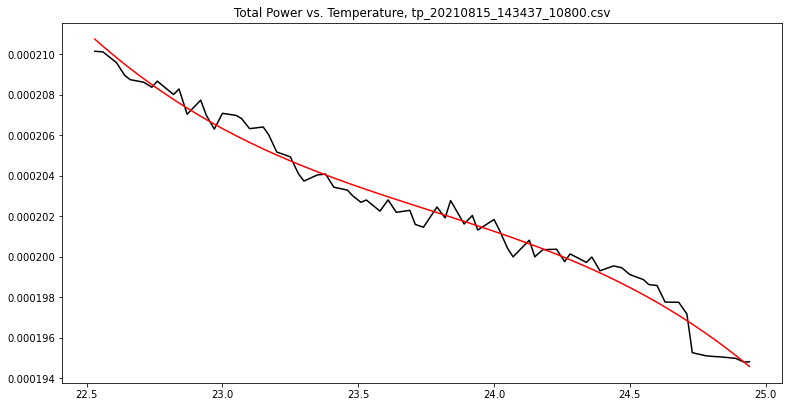
\includegraphics[width=1\textwidth]{tcomp20200818-1.png}
	\label{tcomp:4}
	\caption{The relationship between temperature and power with equivalent 	temperature total power averaging. The curve fit function is shown in 			red.}
\end{figure}

\begin{figure}[h!]
	\centering
	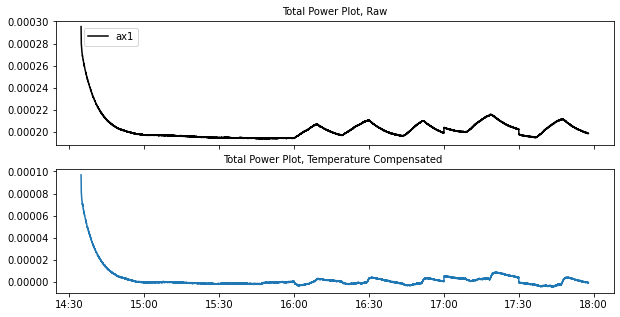
\includegraphics[width=1\textwidth]{tcomp20200818-2.png}
	\label{tcomp:5}
	\caption{Results of temperature compensation after equivalent 					temperature total power averaging applied.}
\end{figure}

The curve fit is noticably better, but the final compensated temperature graph is not. The shape of the graph has changed. It is less smooth than the original algorithm, even with the poorer curve fit. I also tried division instead of subtraction. The curve was identical in shape, just scaled differently.

Looking closely at the graphs, it looks like the bumps of the compensated graph correlate to changes in slope of the original graph. I wonder if there is a temperature respose issue?

I'm not sure what is the true cause is, but I'm considering making my own temperature lookup table. I think I need to set up the cooler experiment, and record temperature changing very slowly.
\\
\end{loggentry}

\end{document}

